\documentclass[sigplan,screen,nonacm]{acmart}
\usepackage{color}
\setlength {\marginparwidth }{2cm}
\usepackage[colorinlistoftodos]{todonotes}
\usepackage[
    type={CC},
    modifier={by-nc-sa},
    version={4.0},
]{doclicense}

%% \BibTeX command to typeset BibTeX logo in the docs
\AtBeginDocument{%
  \providecommand\BibTeX{{%
    \normalfont B\kern-0.5em{\scshape i\kern-0.25em b}\kern-0.8em\TeX}}}

%% end of the preamble, start of the body of the document source.

\begin{document}

%%
%% The "title" command has an optional parameter,
%% allowing the author to define a "short title" to be used in page headers.
\title{Using Internet of Things for Wildlife Tracking}

%% "authornote" and "authornotemark" commands
%% used to denote shared contribution to the research.
\author{Collin R. Beane}
\email{beane039@morris.umn.edu}
\affiliation{%
  \institution{Division of Science and Mathematics
    \\
    University of Minnesota, Morris
  }
  \city{Morris}
  \state{Minnesota}
  \country{USA}
  \postcode{56267}
}

%%
%% The abstract is a short summary of the work to be presented in the
%% article.
\begin{abstract}
  This paper provides a comprehensive examination of the utilization of
  Internet of Things (IoT) devices in wildlife management and tracking,
  their evolutionary trajectory, and practical implementation in data
  acquisition. Central to the discussion are key components of IoT networks,
  including Sigfox, Wi-Fi-enabled devices, and IoT-based wireless sensor
  networks, each analyzed for their role and efficacy. Communication
  modalities within IoT frameworks, coupled with an evaluation of protocol
  performance are evaluated.

  Furthermore, this seminar also addresses challenges inherent in wildlife
  data collection methodologies, such as memory constraints, battery life,
  transmission range and rate, and security vulnerabilities within IoT
  ecosystems. By delving into potential solutions and technological
  advancements, this paper aims to contribute to the refinement of wildlife
  monitoring practices, fostering a more robust and effective approach to
  conservation efforts.
  \todo[inline, color=orange]{This is a preliminary abstract, I mainly added it just so I had something.}
\end{abstract}

\doclicenseThis

\keywords{IoT, networking, Wi-Fi, data transmission, data collection,
  animal trackers, Sigfox, WildFi, Biologging, ecology}


%%
%% This command processes the author and affiliation and title
%% information and builds the first part of the formatted document.
\maketitle

\section{Introduction}
\label{sec:introduction}

\section{Background}
\label{sec:Background}

Comprehending the foundational technology behind the Internet of Things (IoT)
is paramount in grasping its applications in wildlife tracking. This section
aims to furnish a concise overview of biologging, the IoT, and their
intersection in wildlife tracking. Additionally, it will explore current and past
technologies employed in biologging, shedding light on their operational
mechanisms and comparative advantages. By delving into the workings of
traditional wildlife tracking technologies, we can evaluate their merits and
demerits, thereby establishing a framework for evaluating the suitability of
IoT solutions for wildlife tracking.

\subsection{What is Biologging?}
\label{subsec:What is Biologging}

Biologging is a concept that gained popularity in the early 2000's and has continued
to play a pivotal role in understanding animal behavior and ecology. Biologging can be
defined as "The investigation of phenomena in or around free-ranging organisms that are beyond
the boundary of our visibility or experience. \cite{boyd2004bio}"
It is a method of tracking animals in the wild using electronic devices that are
attached to the animal. These devices can be used to track the animal's
movements, monitor its behavior, and collect data on its environment. Biologging
emerged as a powerful tool in ecology in a similar way genomics did for the study
of cell and organ function. The obvious difference being that biologging provides
insights into the behavior and functions of various organisms in environments that
can be hostile or difficult to reach for the observer, rather than the function of cells and
organs \cite{boyd2004bio}. The ability to track animals in their natural environment has
provided researchers with a wealth of data that was previously unattainable. This data
has been used to study animal behavior, migration patterns, and the effects of climate change
on various species\cite{10.3389/fevo.2018.00092}. The data collected from biologging
devices has also been used to inform conservation efforts and to help protect endangered
species \cite{cooke2008biotelemetry}. It is important to understand that biologging is
simply the collection of data from animals in the wild, and it is then up to scientists
or conservationists to use the data to answer questions about the animals or to inform
conservation efforts.

\subsection{What is the Internet of Things?}
\label{subsec:What is the Internet of Things}

The Internet of Things (IoT) represents a transformative shift in the
realm of technology, encompassing a vast array of physical objects empowered
with sensors and software to interact autonomously. These objects collect and
exchange data through network connectivity. In essence, IoT devices, ranging
from commonplace gadgets to sophisticated systems, have the capability to
interface with the internet or communicate wirelessly, thereby facilitating
seamless integration into various facets of daily life. The IoT has been
applied to a wide range of fields, including healthcare, agriculture,
manufacturing, and most important to this paper, wildlife monitoring.
The fundamental structure of an IoT system is comprised of three
interconnected layers: the perception layer, the network layer, and the
application layer\cite{kumar2019internet}. The perception layer is responsible for collecting data
from the environment, which is then transmitted to the application layer via the network layer.
The transmission layer can use a variety of different methods to transmit data, the two most common being
ethernet/WiFi, and cellular networks like 5G and LTE\cite{greengard2021internet}. Lastly, the application
layer is responsible for doing something with the data, such as graph positional data from an
animals GPS sensor. The physical implementation of these layers
can vary greatly, but in general, the perception layer consists of a sensor or device that can
output a signal to be received by a gateway device(the most common gateway device for
the average person would be a wireless router). The gateway device is connected to
the internet using one of the aforementioned methods, and it is responsible for
receiving the data from the perception layer device and transmitting it to the application
layer, which could be a database to store the data, or a web application to display
the data\cite{kumar2019internet}. These three theoretical layers are important in understanding the IoT,
and how it can be used in wildlife tracking. The Wild-Fi biologging tag, which will be
discussed later in this paper, is a prime example of how these three layers are implemented
in a biologging device and is visually explained by figure ~\ref{fig:wild-fi_IoT_diagram}.
\begin{figure}[htbp]
  \centering
  \fbox{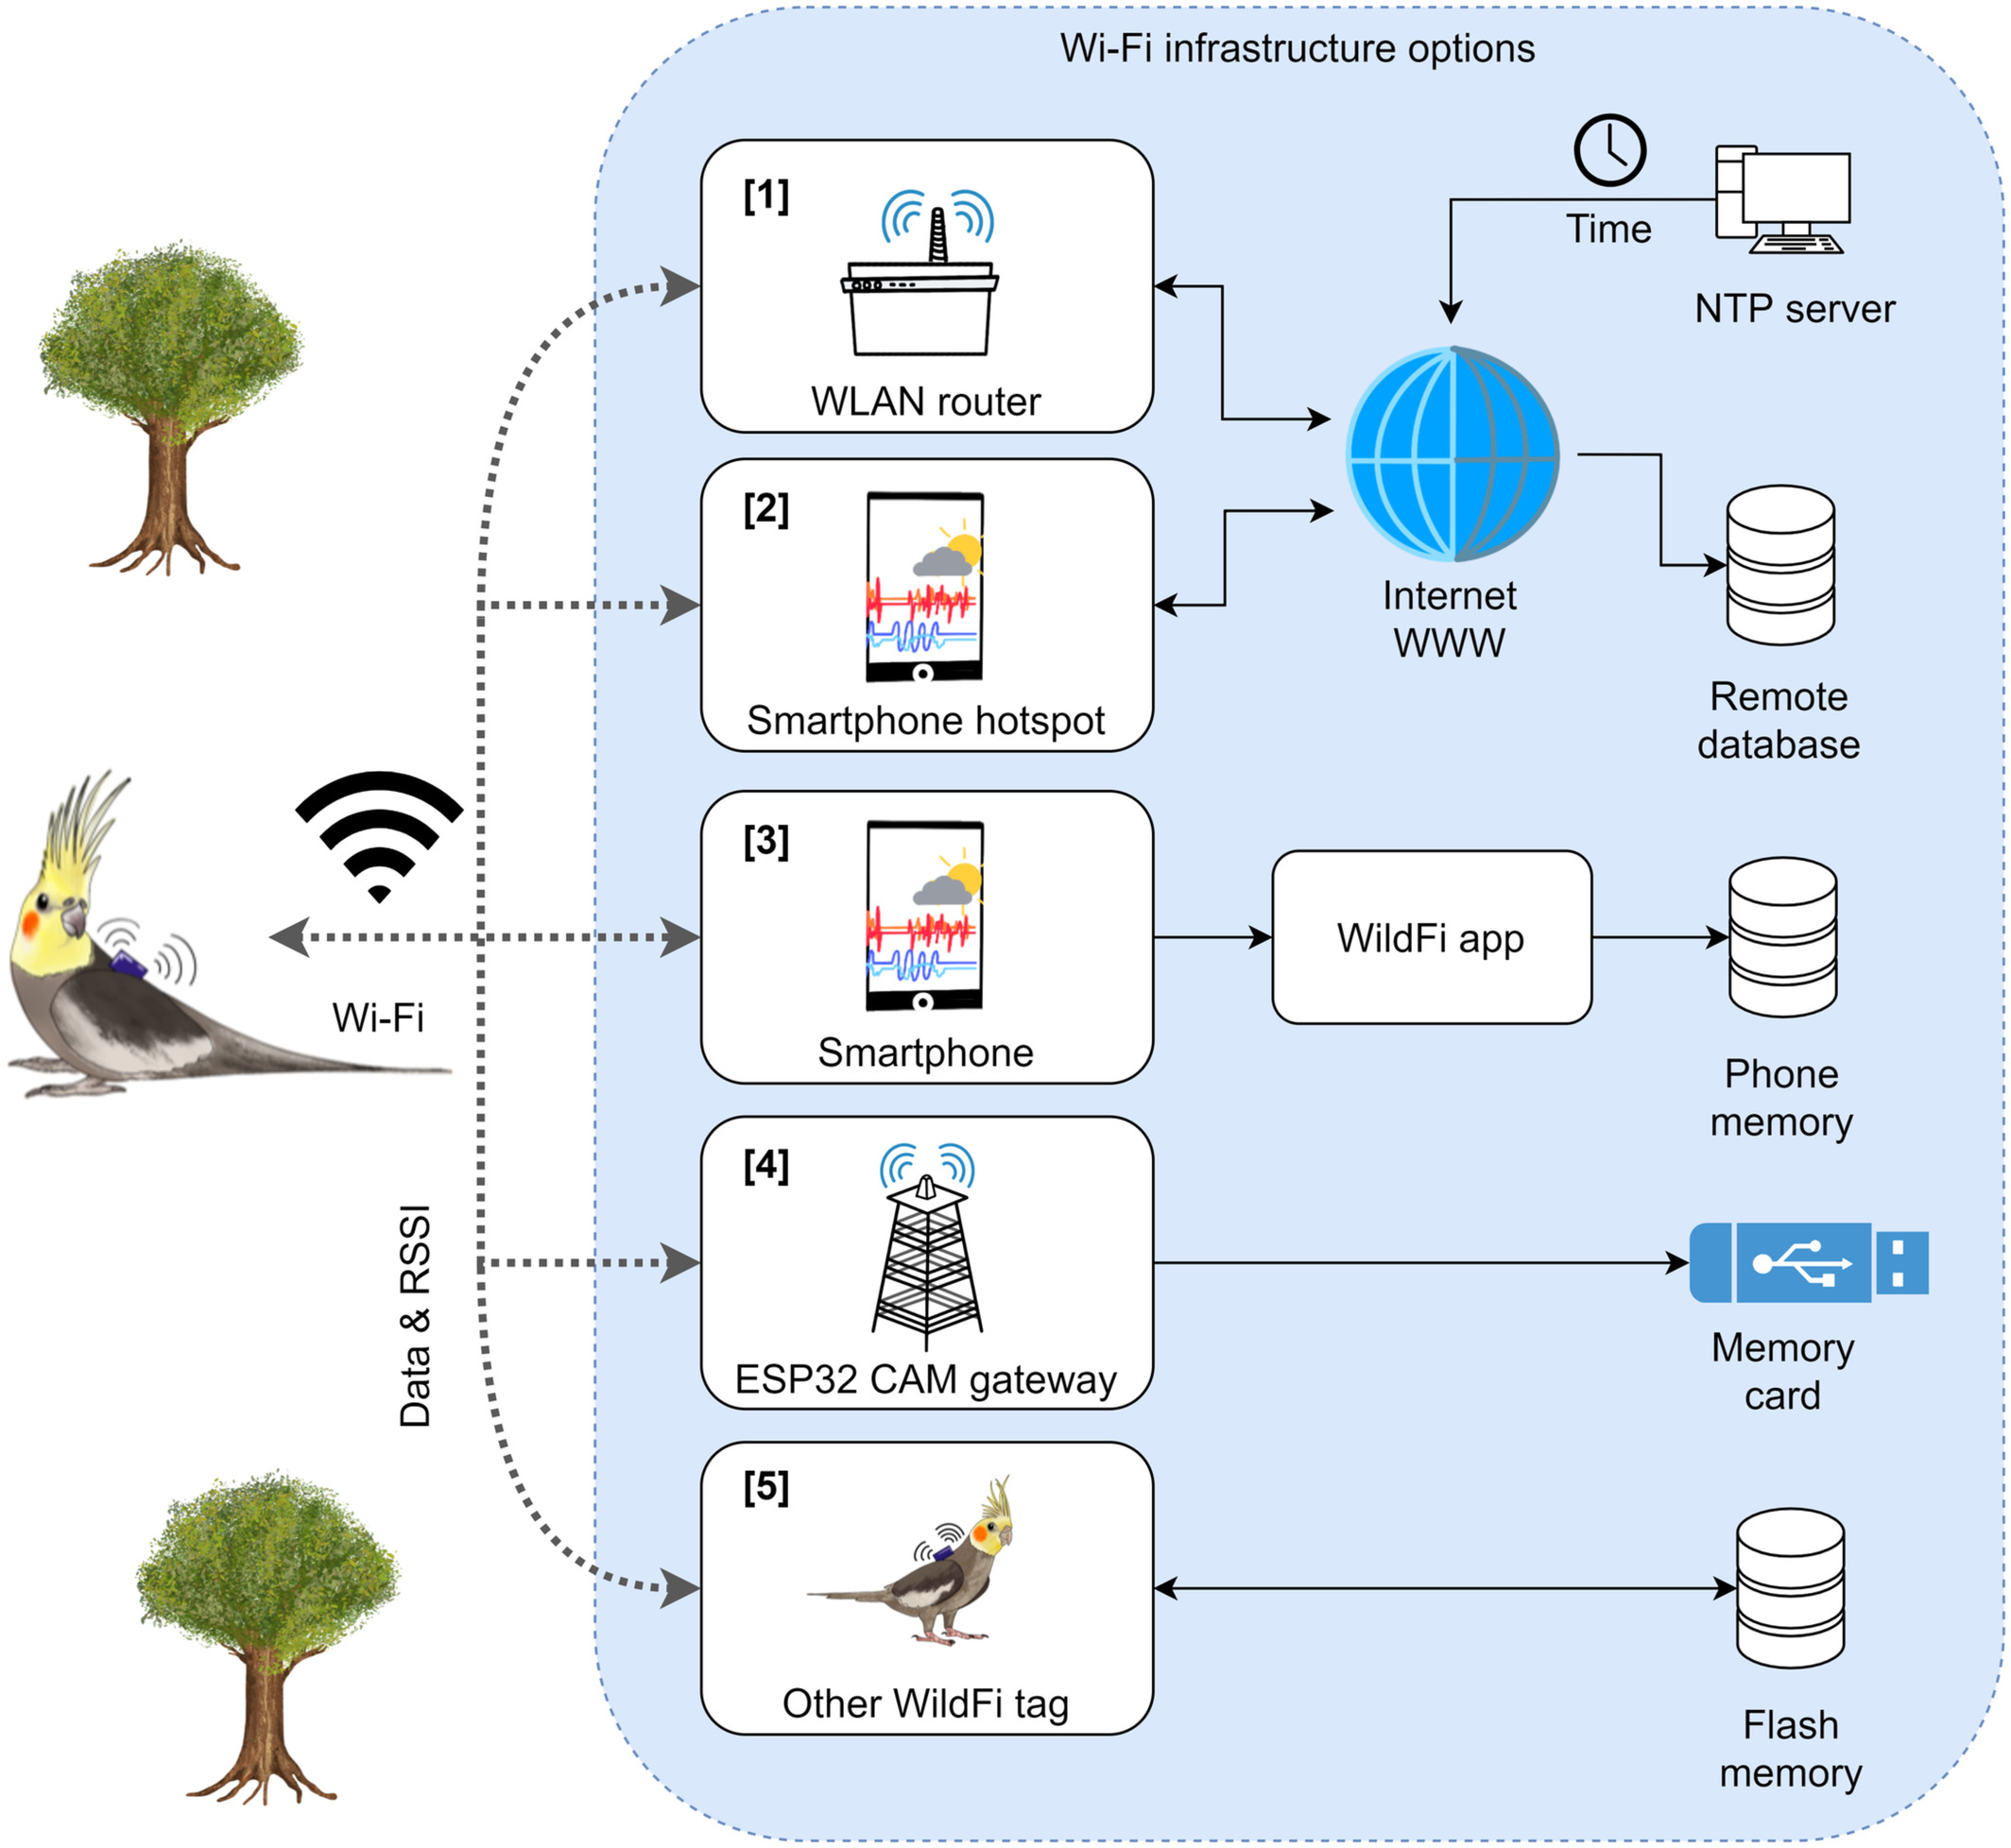
\includegraphics[width=.9\columnwidth]{WildFi_IoT.jpg}}
  \caption{Wild-fi IoT infrastructure overview}
  \label{fig:wild-fi_IoT_diagram}
\end{figure}
\todo[inline, color=orange]{Include citation for the figure.}


\subsection{What are the Other Biologging Methods?}
\label{subsec:What are the Other Biologging Methods?}

Various stratagies have been used in the past to track animals in the wild. Many
implement variations of the same technology within the tracking sensors;
GPS, accelerometers, and magnetometers are the most common sensors used in
biologging devices. These data from these sensors help researchers understand
the animal's  speed, direction, and position, which allows for a 3D mapping of
positions\cite{Kidangoor_2024}. The compilation of this data can be seen in Figure ~\ref{fig:prairie_dog_3D_movement}
from the Smithsonian's National Zoo and Conservation Biology Institute, which
shows the 3D movement of a prairie dogs.
\begin{figure}[htbp]
  \centering
  \fbox{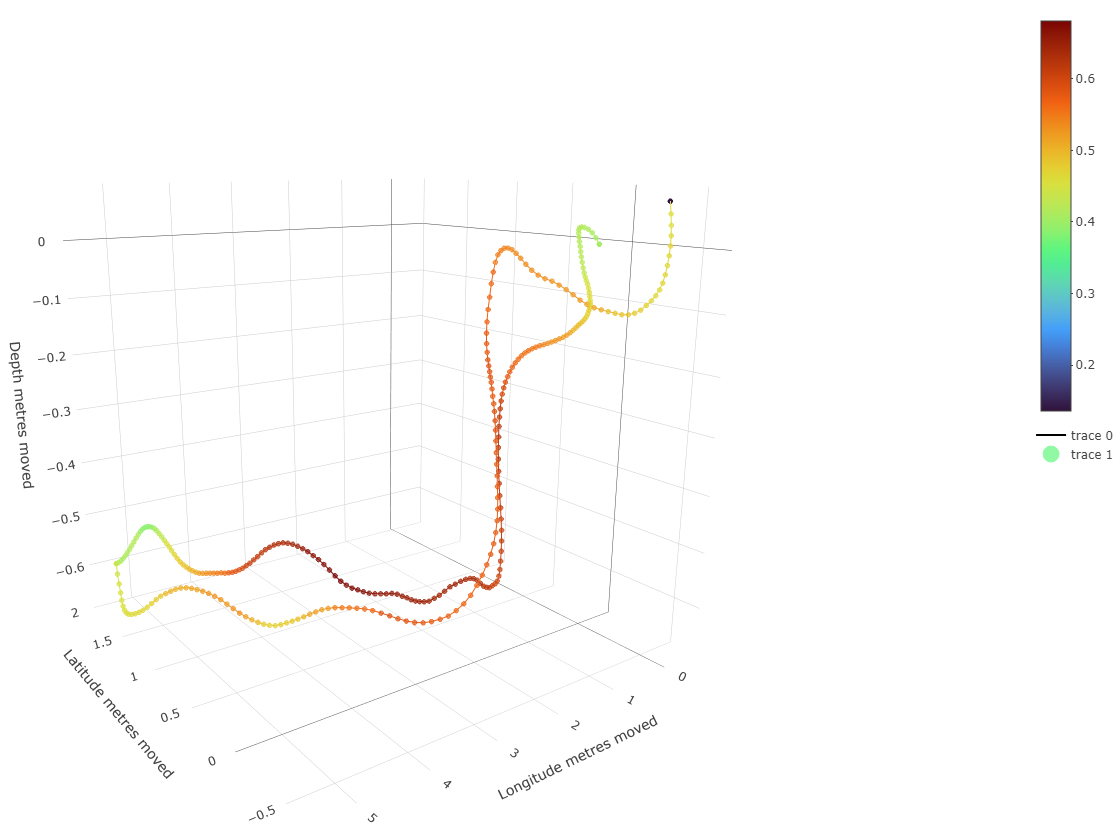
\includegraphics[width=.9\columnwidth]{prairie_dog_map.jpg}}
  \caption{3D movement of a prairie dog}
  \label{fig:prairie_dog_3D_movement}
\end{figure}
\todo[inline, color=orange]{Include citation for the figure.}
Most biologging trackers will implement these types of sensors, but the
implementation of these sensors can vary greatly. More importantly, the
communication of the data from these sensors can vary greatly. One of the
most popular methods for transmitting data is the use of cellular networks.
A study conducted by a professor from UC Irvine tested the use of cellular
networks to analyze the pollution levels in the San Jose area by using pigeons
equipped with GPS and automotive emissions sensors \cite{Martin_2006}. Professor
Da Costa had to pay about 10 cents for each message transmitted, and two
messages are sent every minute by each pigeon\cite{Martin_2006}. This leads into one of the biggest
disadvantages of using cellular networks: cost. Another obvious disadvantage
is that cellular networks are not available in all areas, and the range of
cellular networks is limited. It is also practically impossible for researchers
to improve the range of cellular networks by adding more cell towers to cover
their study area. Radio frequency is another technology that has been used to
transmit data from biologging devices for decades. The use of radio frequency
to transmit data from biologging devices requires a receiver to be within range
of the transmitter, and the range of the transmitter is limited by the power of
the transmitter and the frequency of the radio waves. The receiver and transmitter
used by Cooke et al. on marine animals had an effective range of 5 to 1000m and 
is only able to transmit periodic tracking records or time stamped data from loggers
\cite{cooke2012biotelemetry}. This falls short of the capabilities of IoT enabled 
biologging devices using LPWAN networks, which are able to transmit data in real time, and can transmit 
data over much longer distances. 

\section{Components of a IoT Biologging System}
\label{sec:Components of a IoT Biologging Device}

\subsection{The Sensor Device}
\label{subsec:The Sensor Device}


\section{Data Transmission}
\label{sec:Data Transmission}

\section{Networking Protocols}
\label{sec:Networking Protocols}

The networking of a IoT based biologging system is crucial in ensuring safe and
efficient data transmission. The networking protocols used in a biologging system
are responsible for transmitting data from the sensor device to the application
layer, and they are also responsible for ensuring that the data is transmitted
safely and securely. The two most popular types of networking protocols used in
biologging systems are Low Power Wide Area Networks (LPWAN) and Cellular Networks.
These two types of networks have their own advantages and disadvantages, and
the choice of which network to use is dependent on the specific use case. No
matter what method is used, the networking protocols used in a biologging system
must be able to transmit data over long distances, and they must be able to
transmit data in a secure way. The security of the data is especially important
in a biologging system, as the data being transmitted is often sensitive and
can be used to track the location of an animal, which in the hand of an illegal
hunter, could be disastrous.

\subsection{Low Power Wide Area Networks (LPWAN)}
\label{subsec:Low Power Wide Area Networks (LPWAN)}

\subsection{Cellular Networks}
\label{subsec:Cellular Networks}

\subsection{Protocol Comparison and Selection Criteria}
\label{subsec:Protocol Comparison and Selection Criteria}

\subsection{Security Protocols}
\label{subsec:Security Protocols}
%SLP Protocols

\section{Challenges to Overcome}
\label{sec:Challenges to Overcome}


%%
%% The acknowledgments section is defined using the "acks" environment
%% (and NOT an unnumbered section). This ensures the proper
%% identification of the section in the article metadata, and the
%% consistent spelling of the heading.
\begin{acks}
  This is where you thank those who helped you better understand the material
  and gave you helpful feedback on the paper, usually including your adviser.
  This is not a place to thank your family, your significant other or your best friend,
  or anyone else  for moral support or yummy cookies.
\end{acks}

%%
%% The next two lines define the bibliography style to be used, and
%% the bibliography file.
\bibliographystyle{ACM-Reference-Format}
\bibliography{CBeaneSeniorSem}


\end{document}
\endinput
%%
%% End of file `sample-sigplan.tex'.
